\chapter{Electronics}

This chapter describes the electronic components.
The head node and compute nodes are off-the-shelf embedded systems and require little to no hardware related modifications.

There are 2 custom PCB designs: the compute node power board (\textit{ccpad}) and the panel power distribution board (\textit{ccpdu}).

Software:

\begin{itemize}
	\item \href{http://kicad-pcb.org/}{KiCad}
\end{itemize}

\section{NanoPC-T4}

See \url{https://www.friendlyarm.com/index.php?route=product/product&product_id=225}.

\section{NanoPi M4 2 GB}

See \url{https://www.friendlyarm.com/index.php?route=product/product&product_id=234}.

\section{ccpad}

The main purpose of a ccpad is to supply a compute node with power.
While a compute node can be powered via USB Type-C, the USB Type-C cables / connectors are relatively expensive and their length make them non-ideal for this build.

A ccpad has an input terminal for 5 V and is connected directly to the pin header of a compute board.
This setup also allows for a power measurement IC to be added \emph{and connected} to a compute board.

An \textit{INA219 Zero-Drift, Bidrectional Current/Power Monitor with I²C Interface} is used.

Pin header connector and input terminal are installed on \emph{the same side}.

Consider covering up the bottom of the board with hot glue to prevent short circuits with the adjacent V-Mount panel when fully assembled.

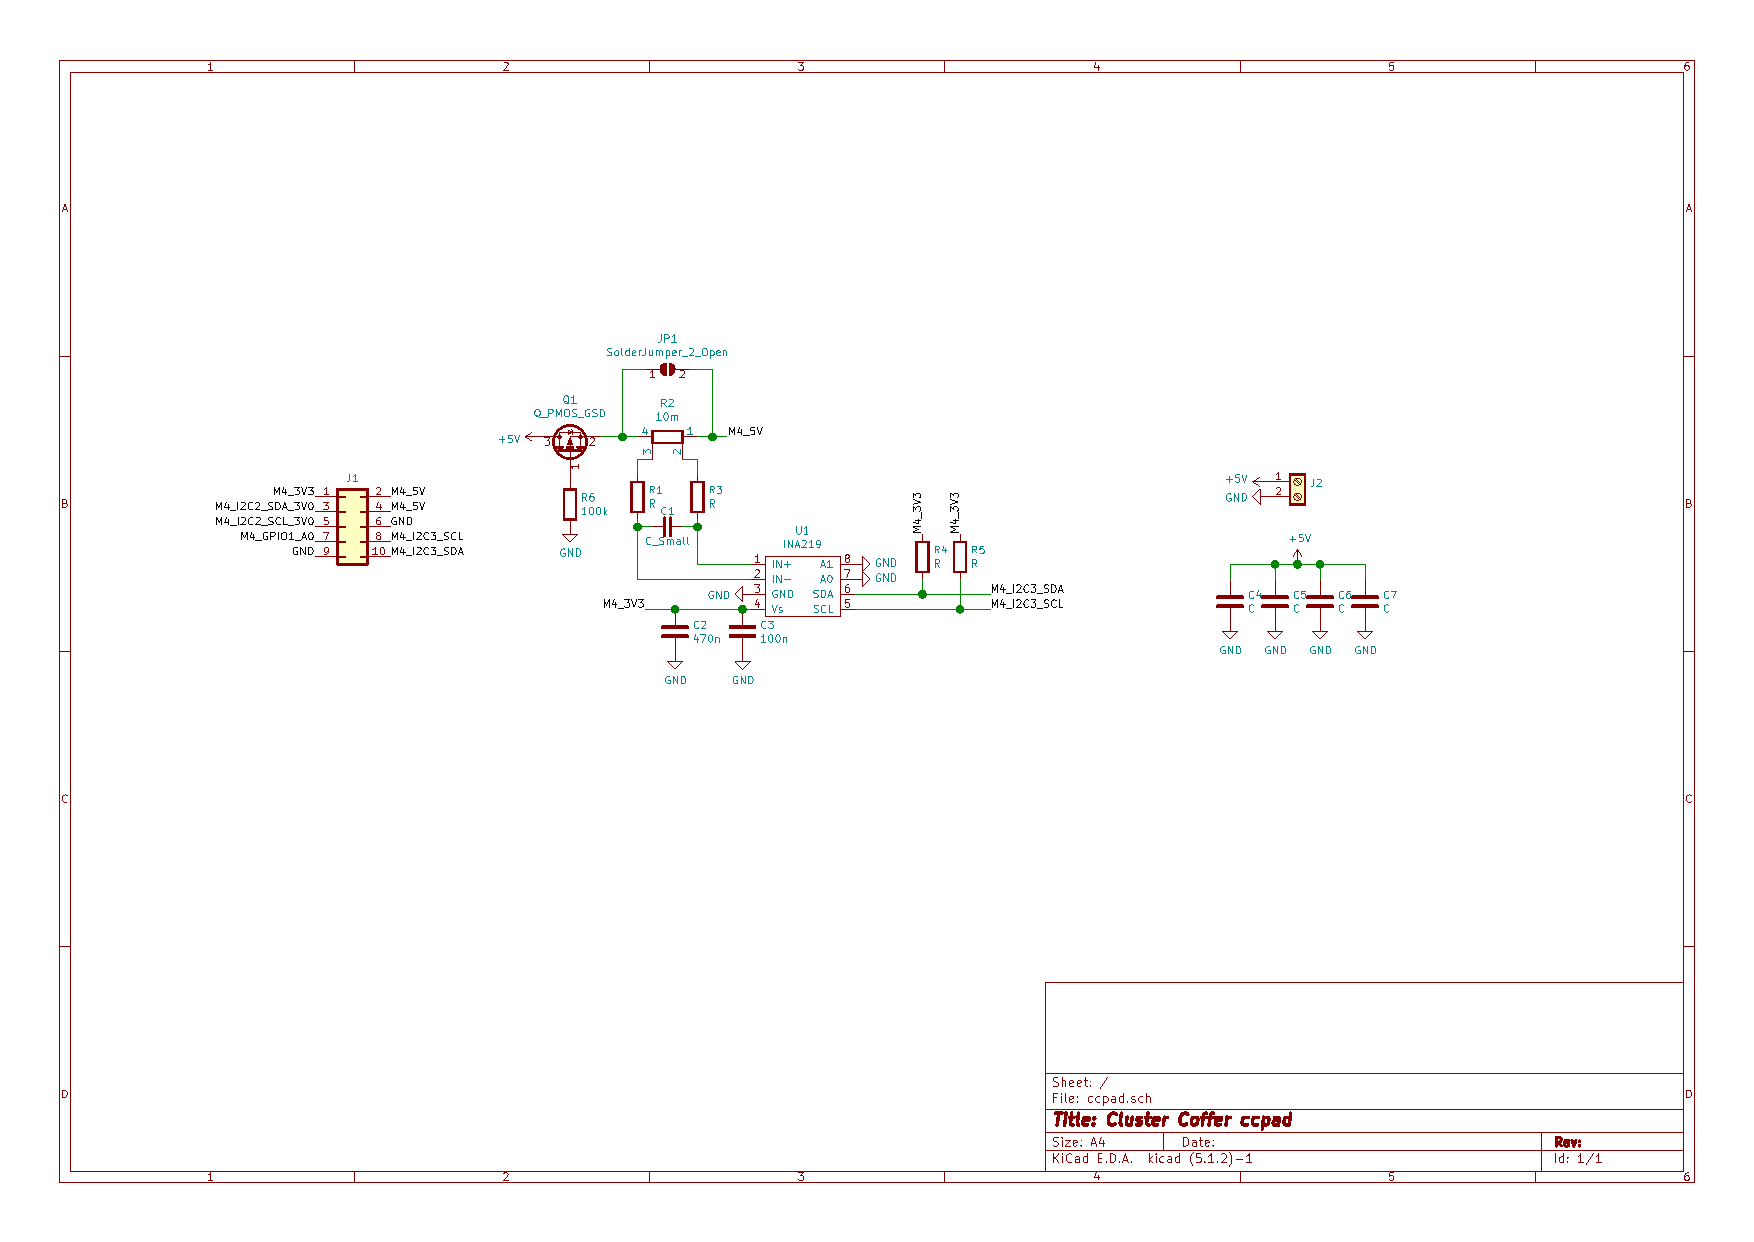
\includepdf[fitpaper]{inc/ccpad_schematic.pdf}
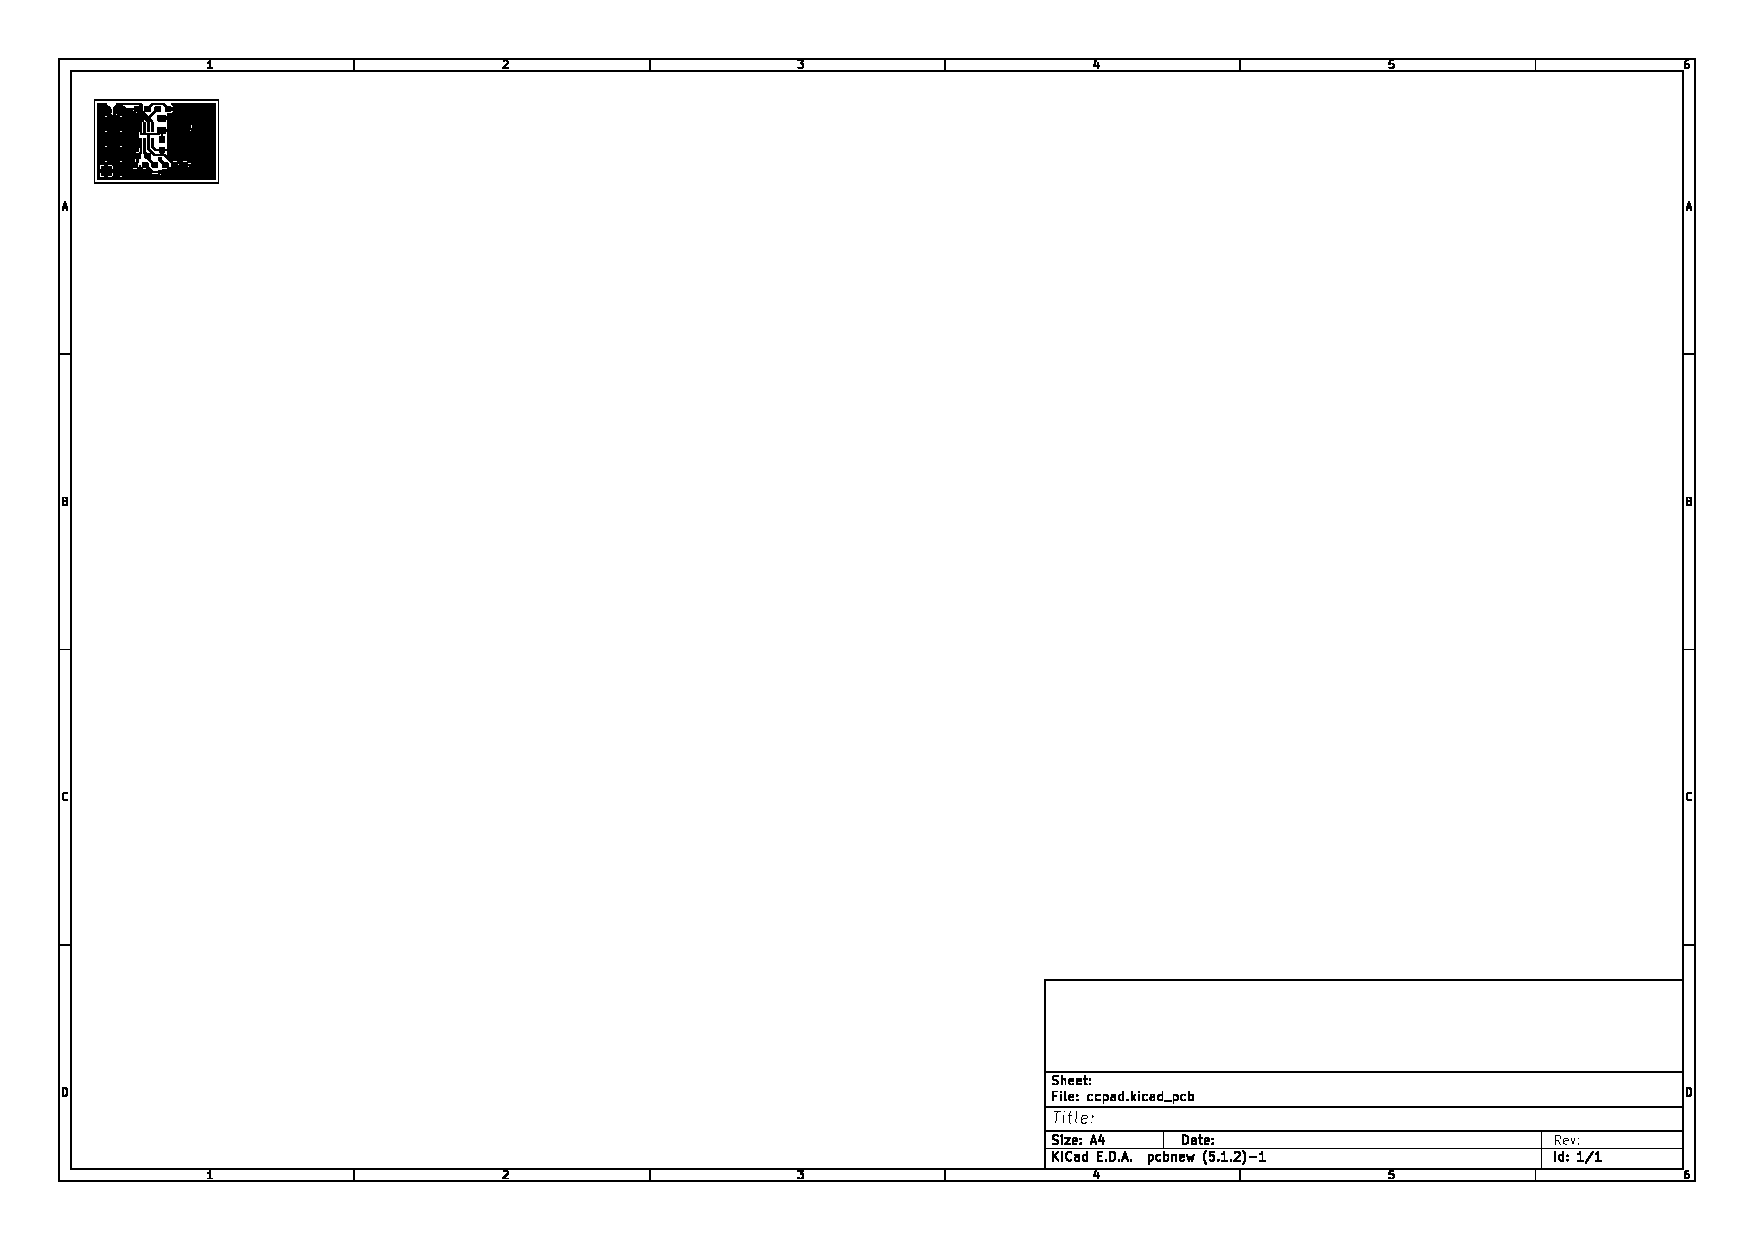
\includepdf[fitpaper]{inc/ccpad_top.pdf}
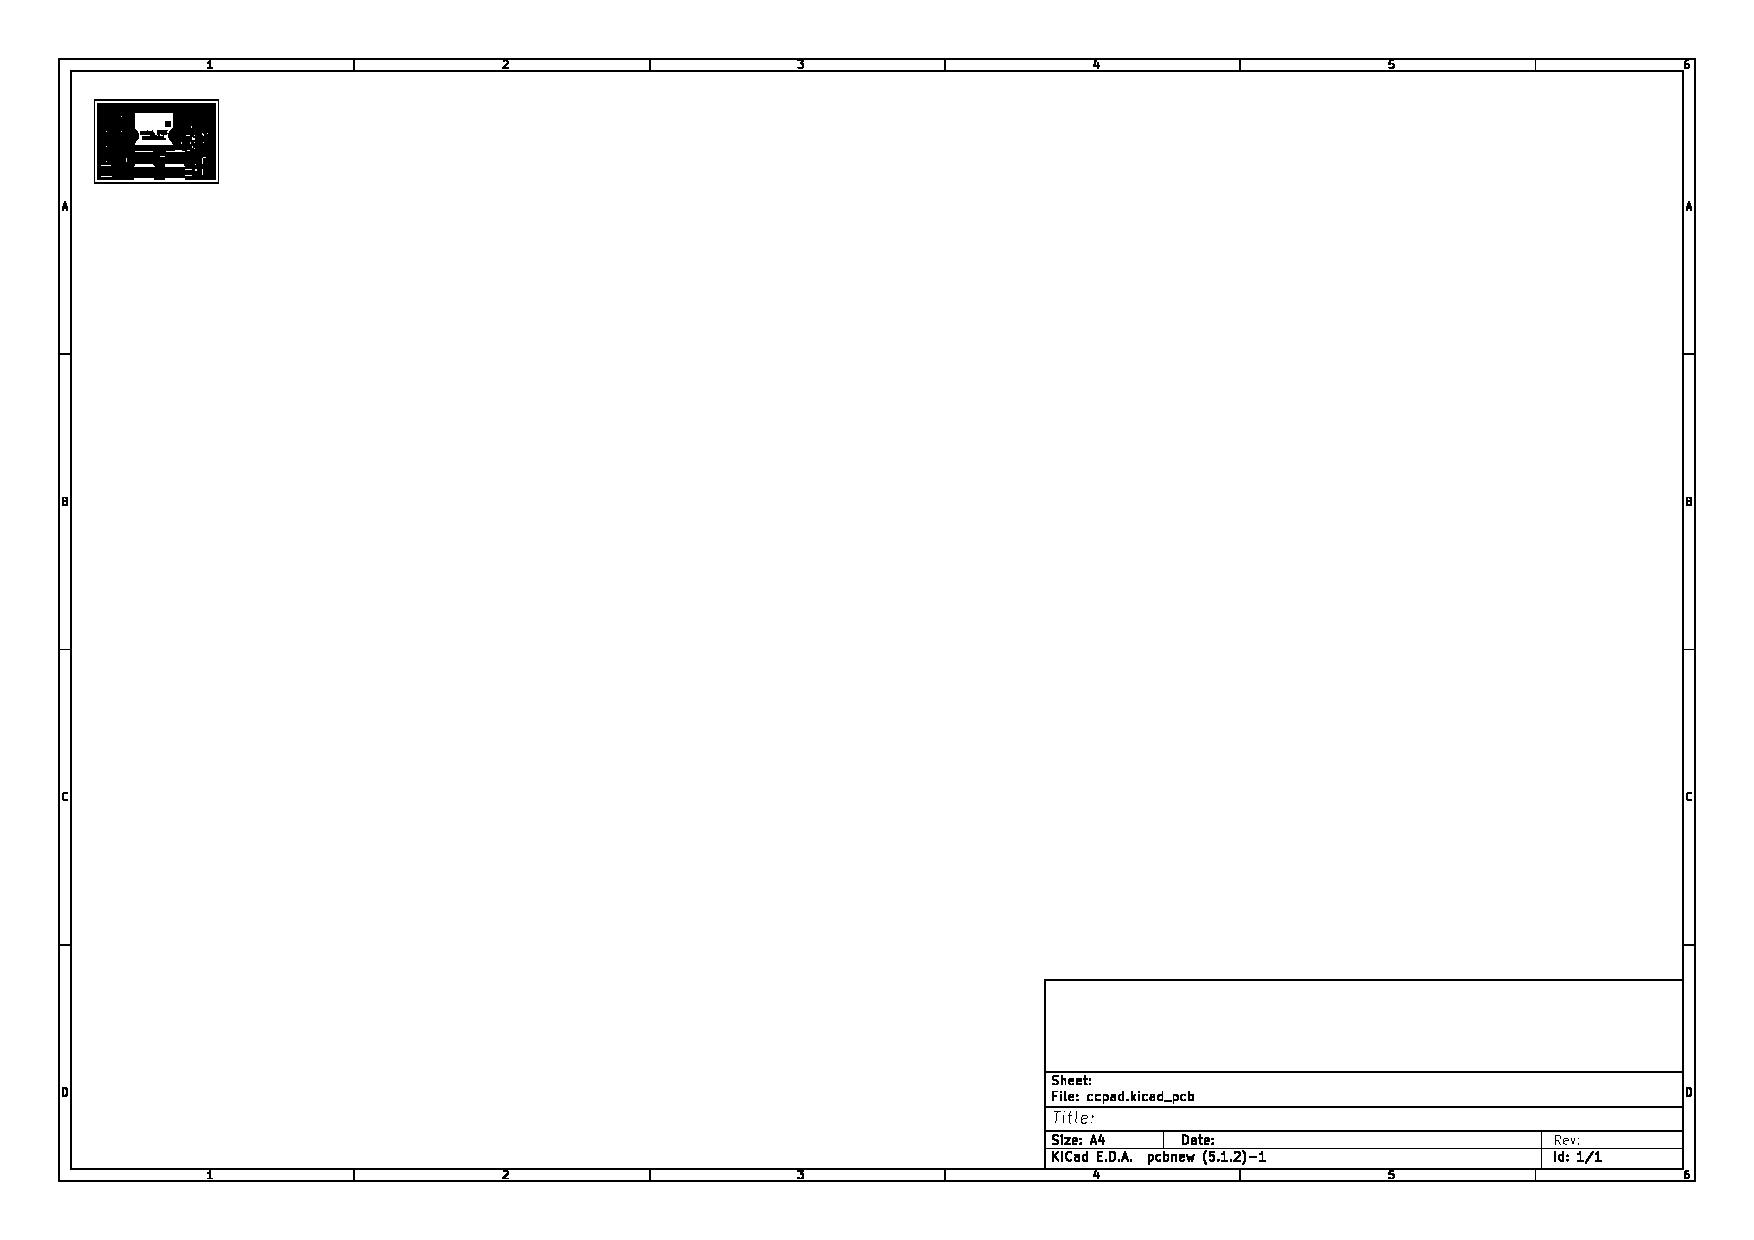
\includepdf[fitpaper]{inc/ccpad_bottom.pdf}
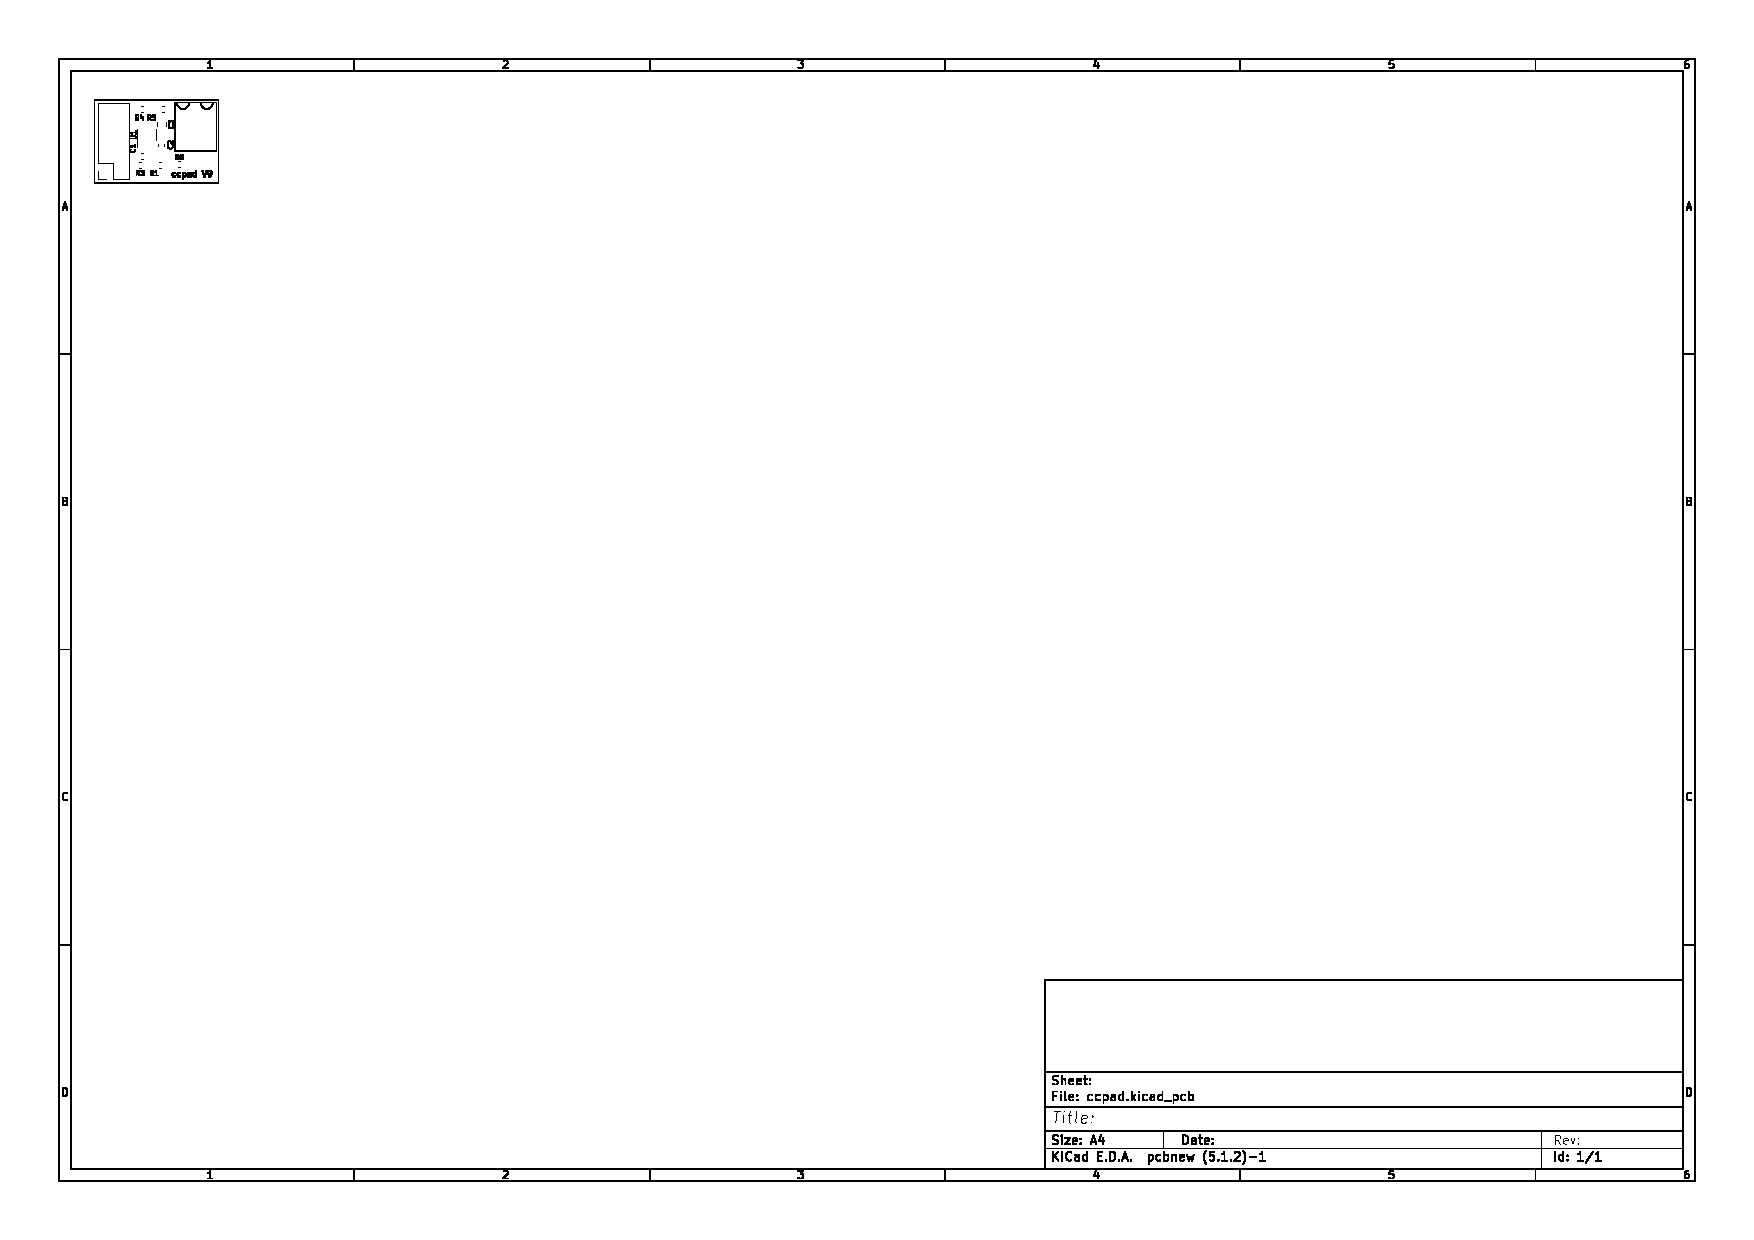
\includepdf[fitpaper]{inc/ccpad_silk.pdf}
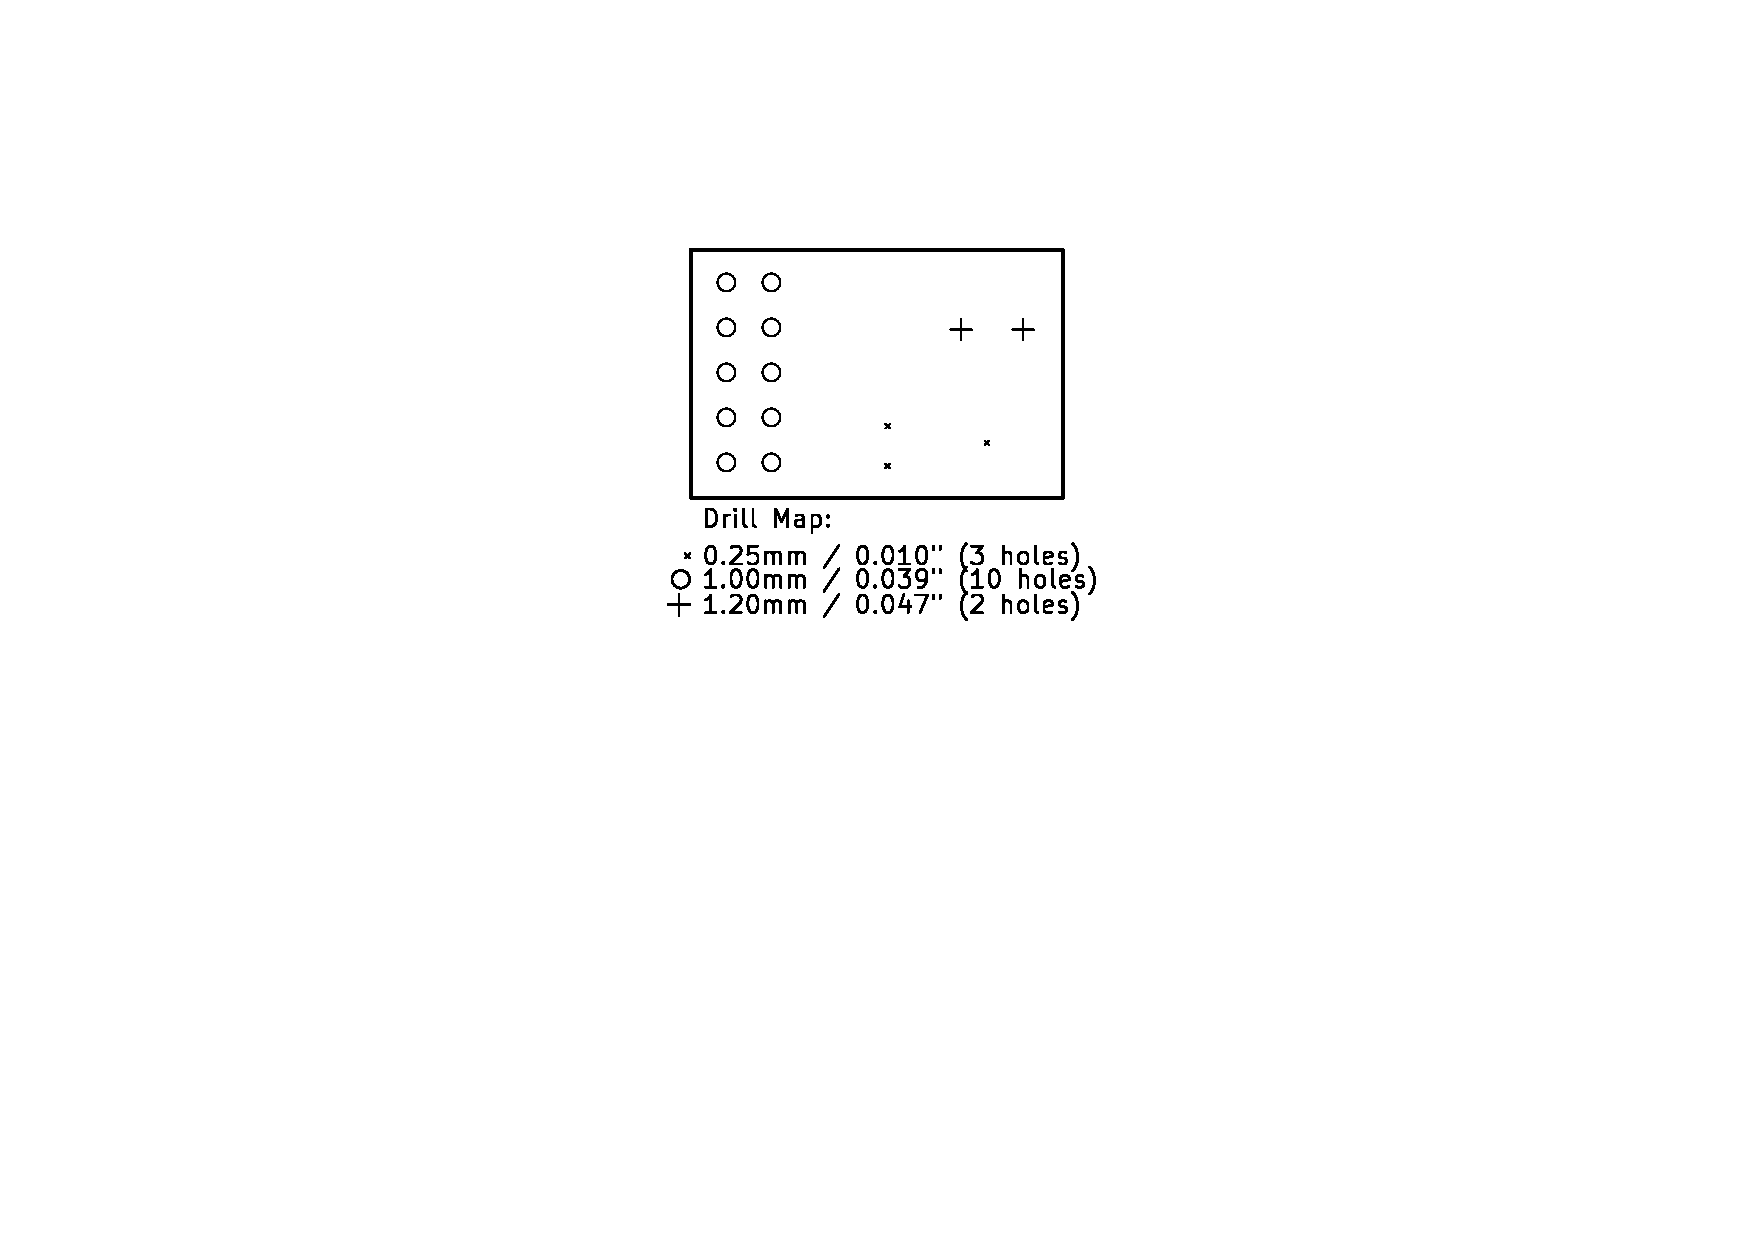
\includepdf[fitpaper]{inc/ccpad_drill.pdf}

\section{ccpdu}

The ccpdu serves as a power distribution board.
While the fans run with 12 V, the compute nodes require 5 V.

The four toggle switches per board are used to mechanically mount it to the V-Mount panel.
Switches and terminals are installed on \emph{opposite sides}.

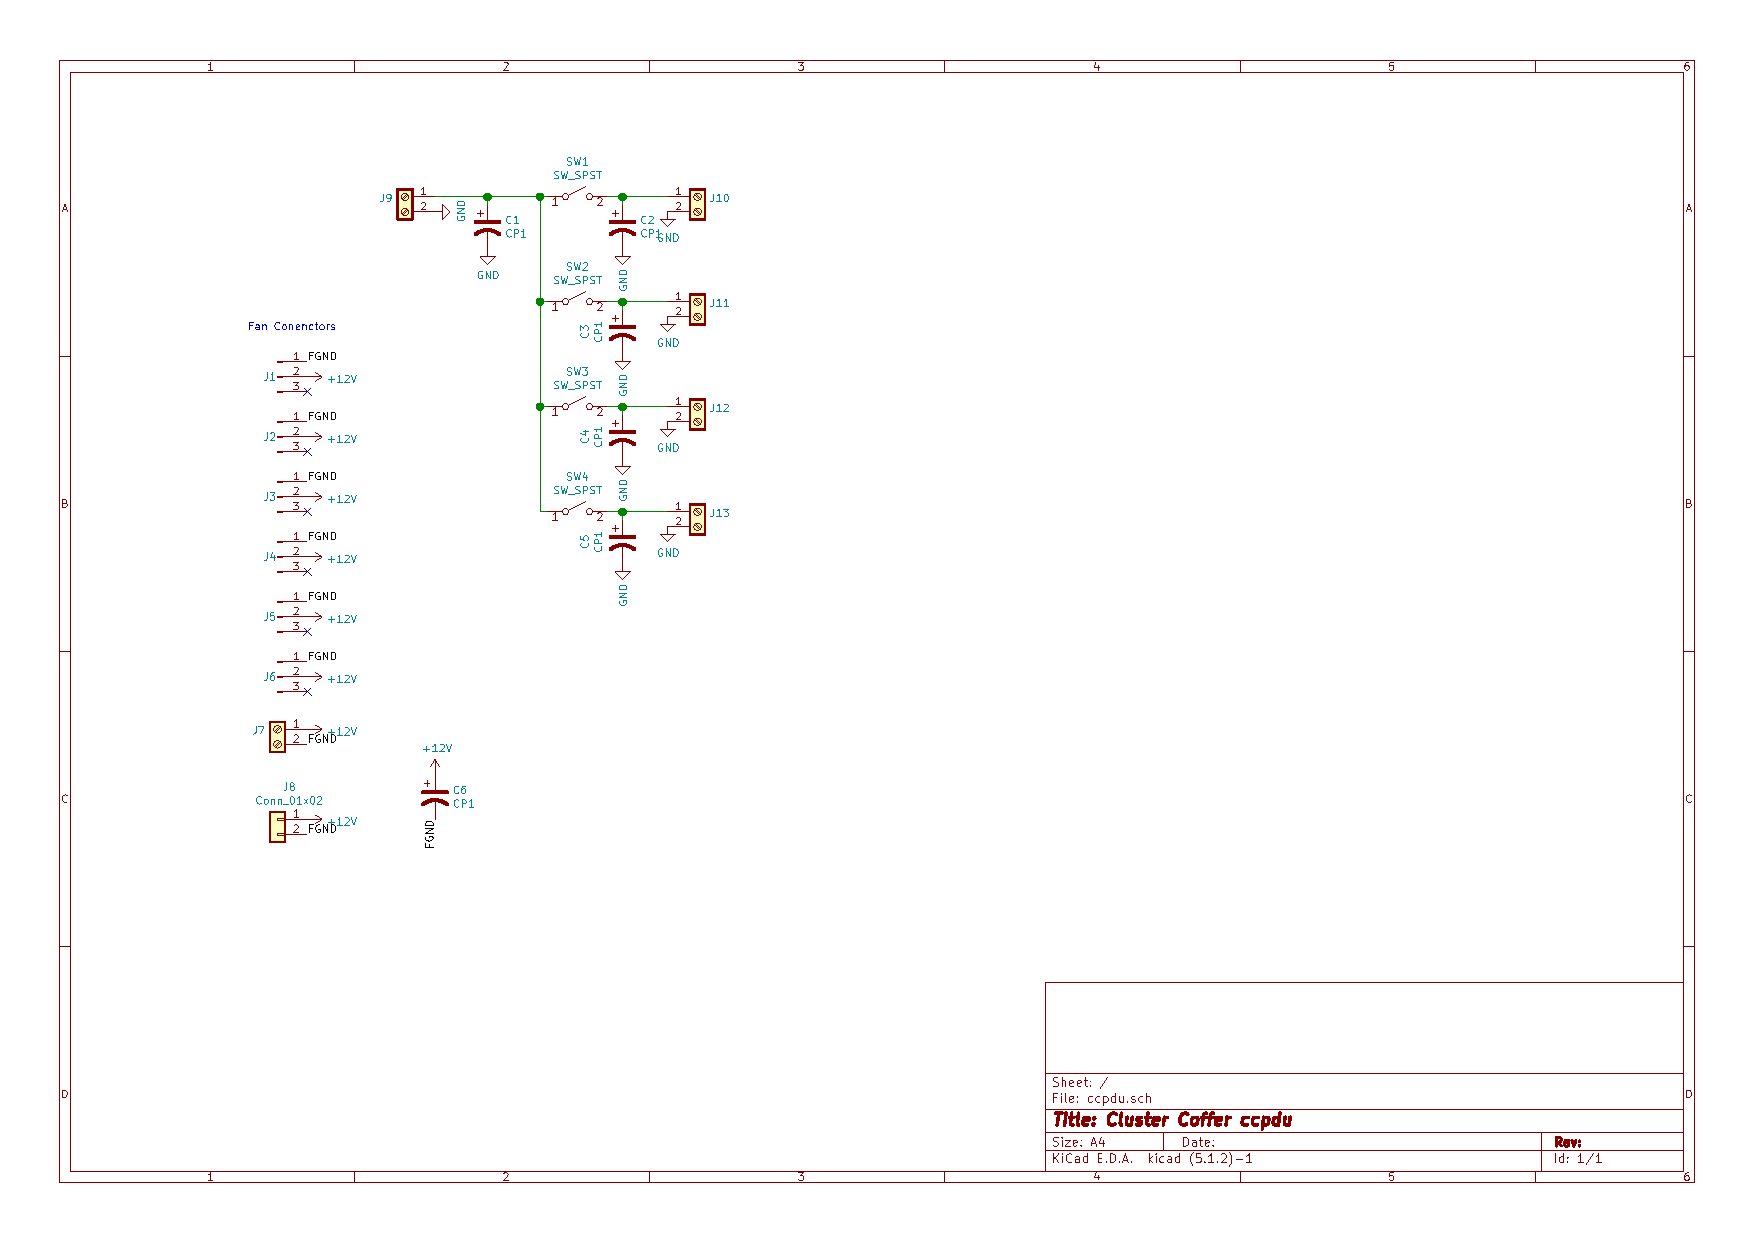
\includepdf[fitpaper]{inc/ccpdu_schematic.pdf}
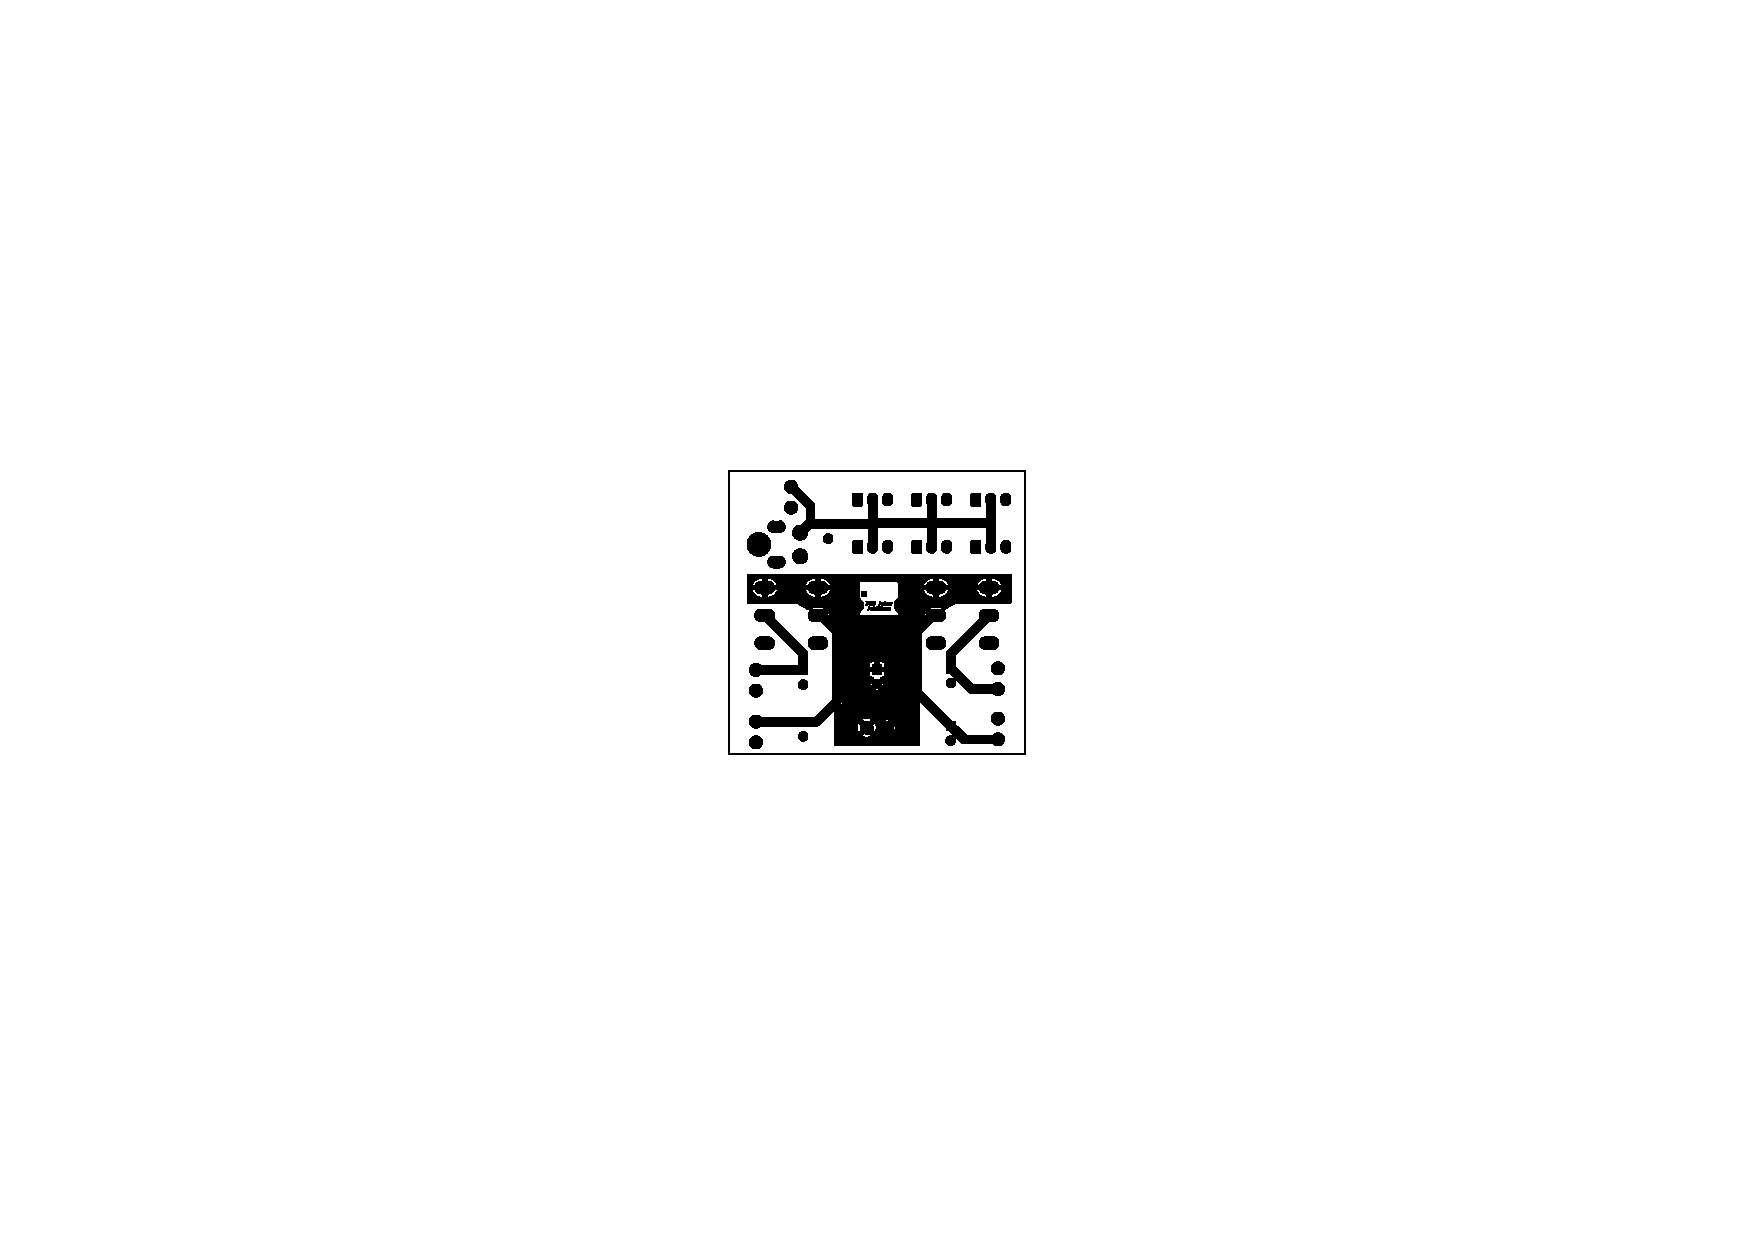
\includepdf[fitpaper]{inc/ccpdu_top.pdf}
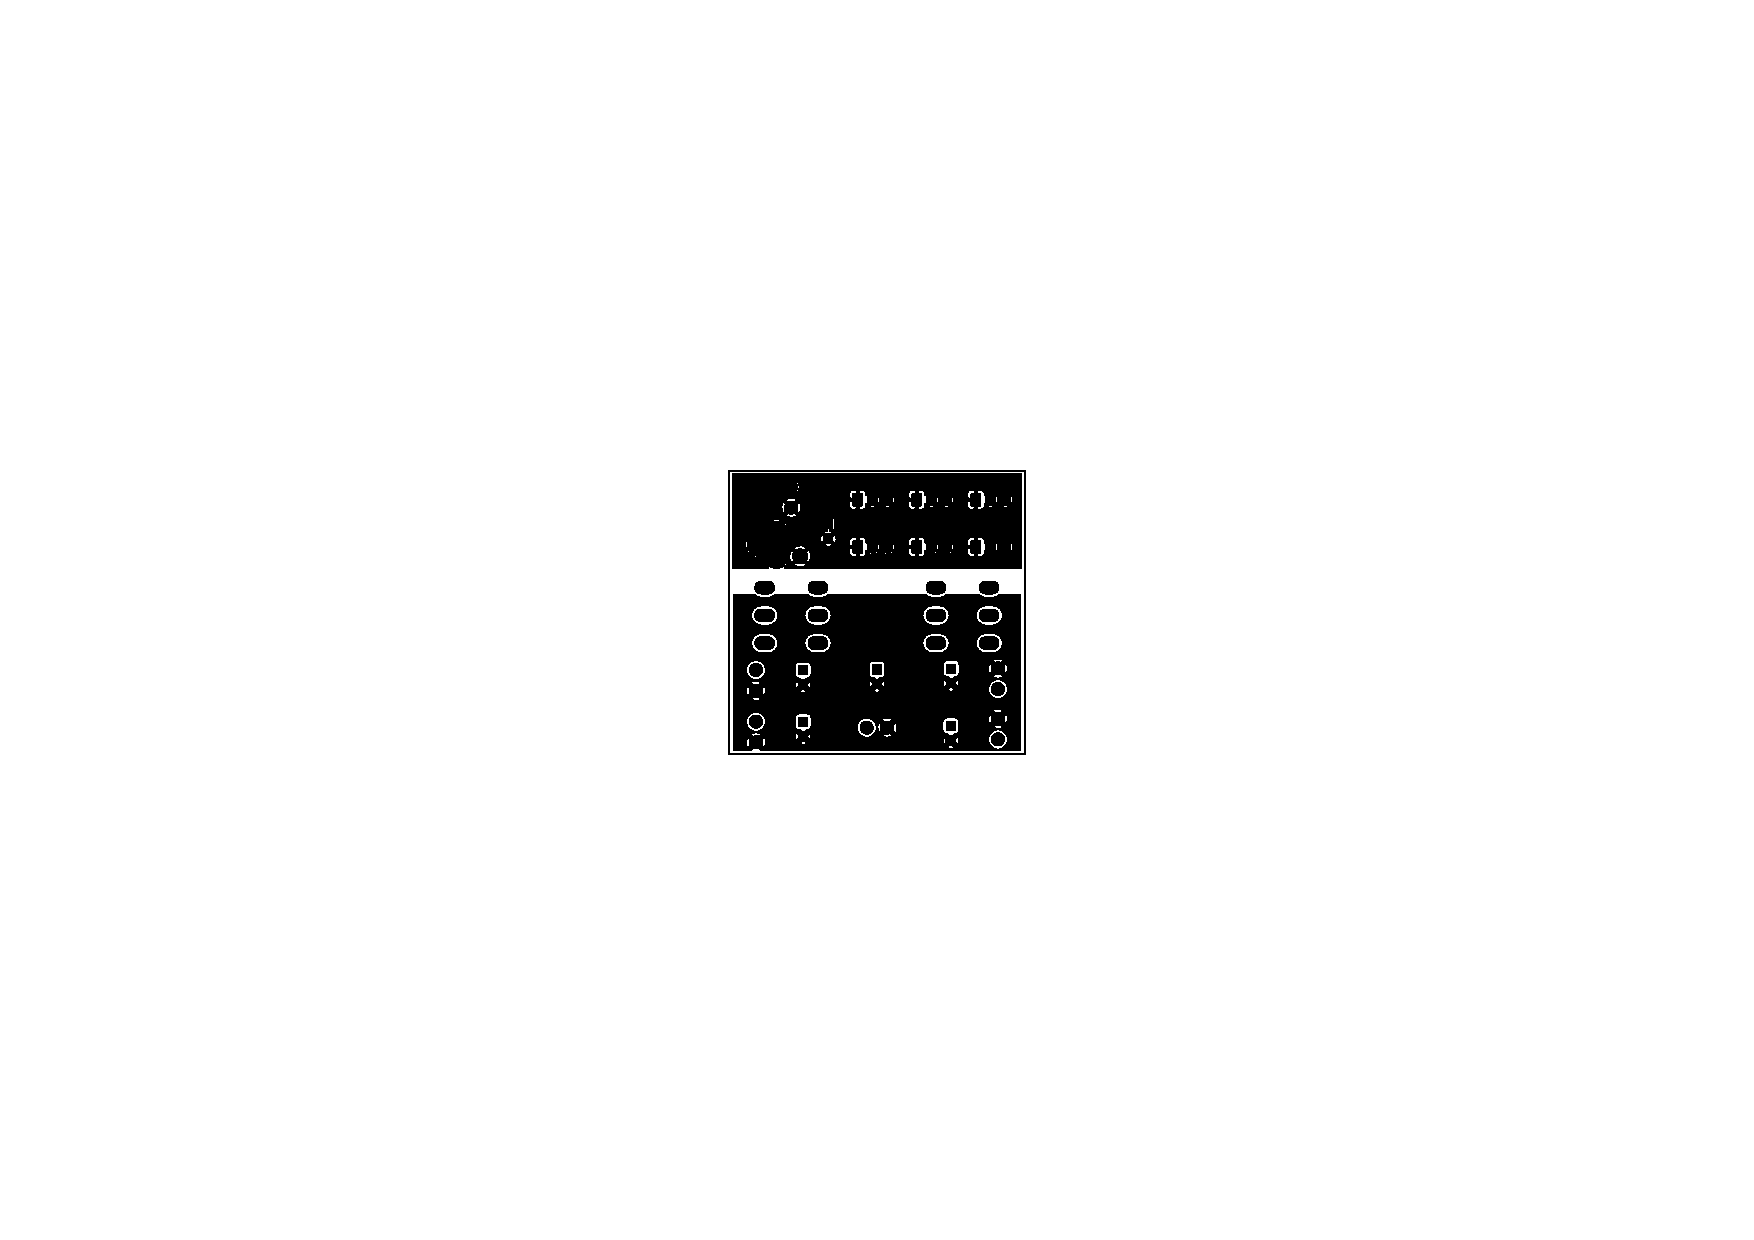
\includepdf[fitpaper]{inc/ccpdu_bottom.pdf}
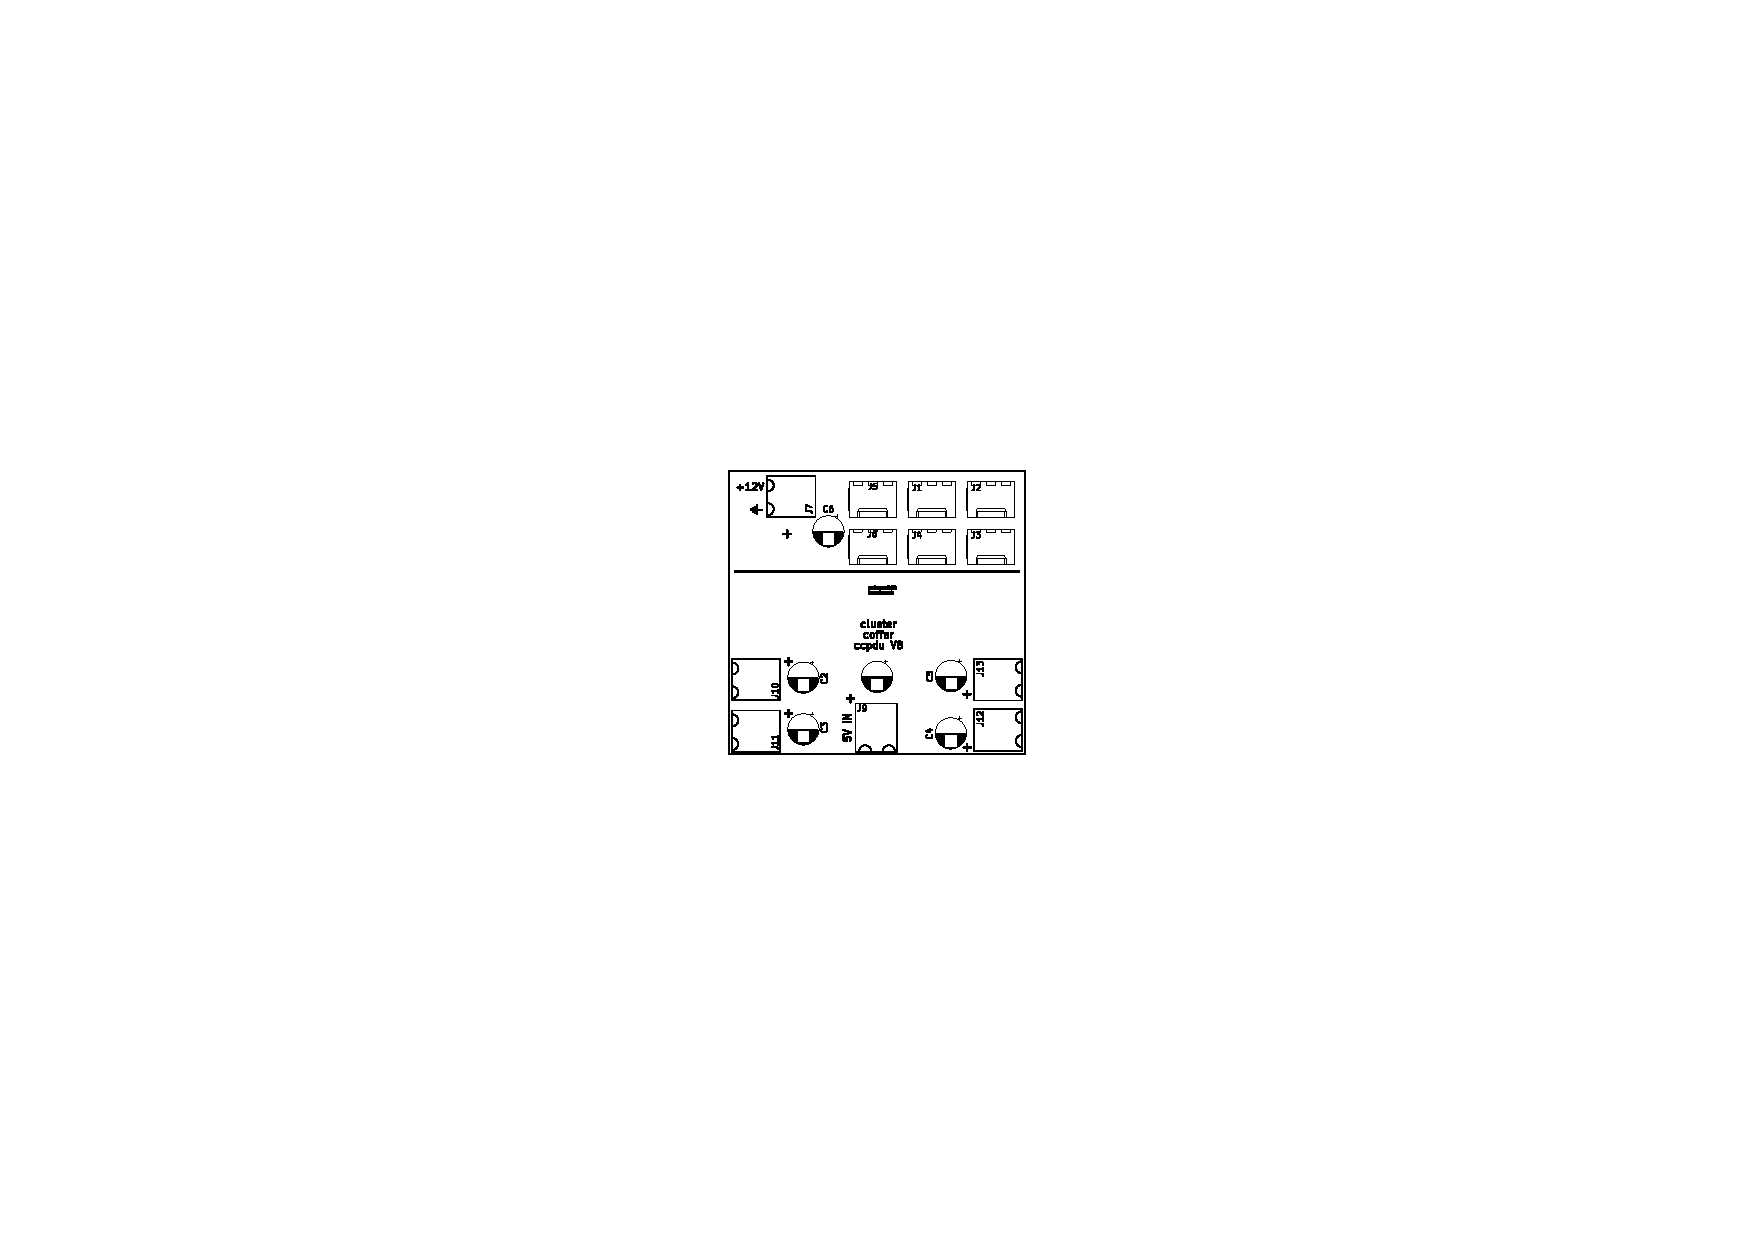
\includepdf[fitpaper]{inc/ccpdu_silk.pdf}
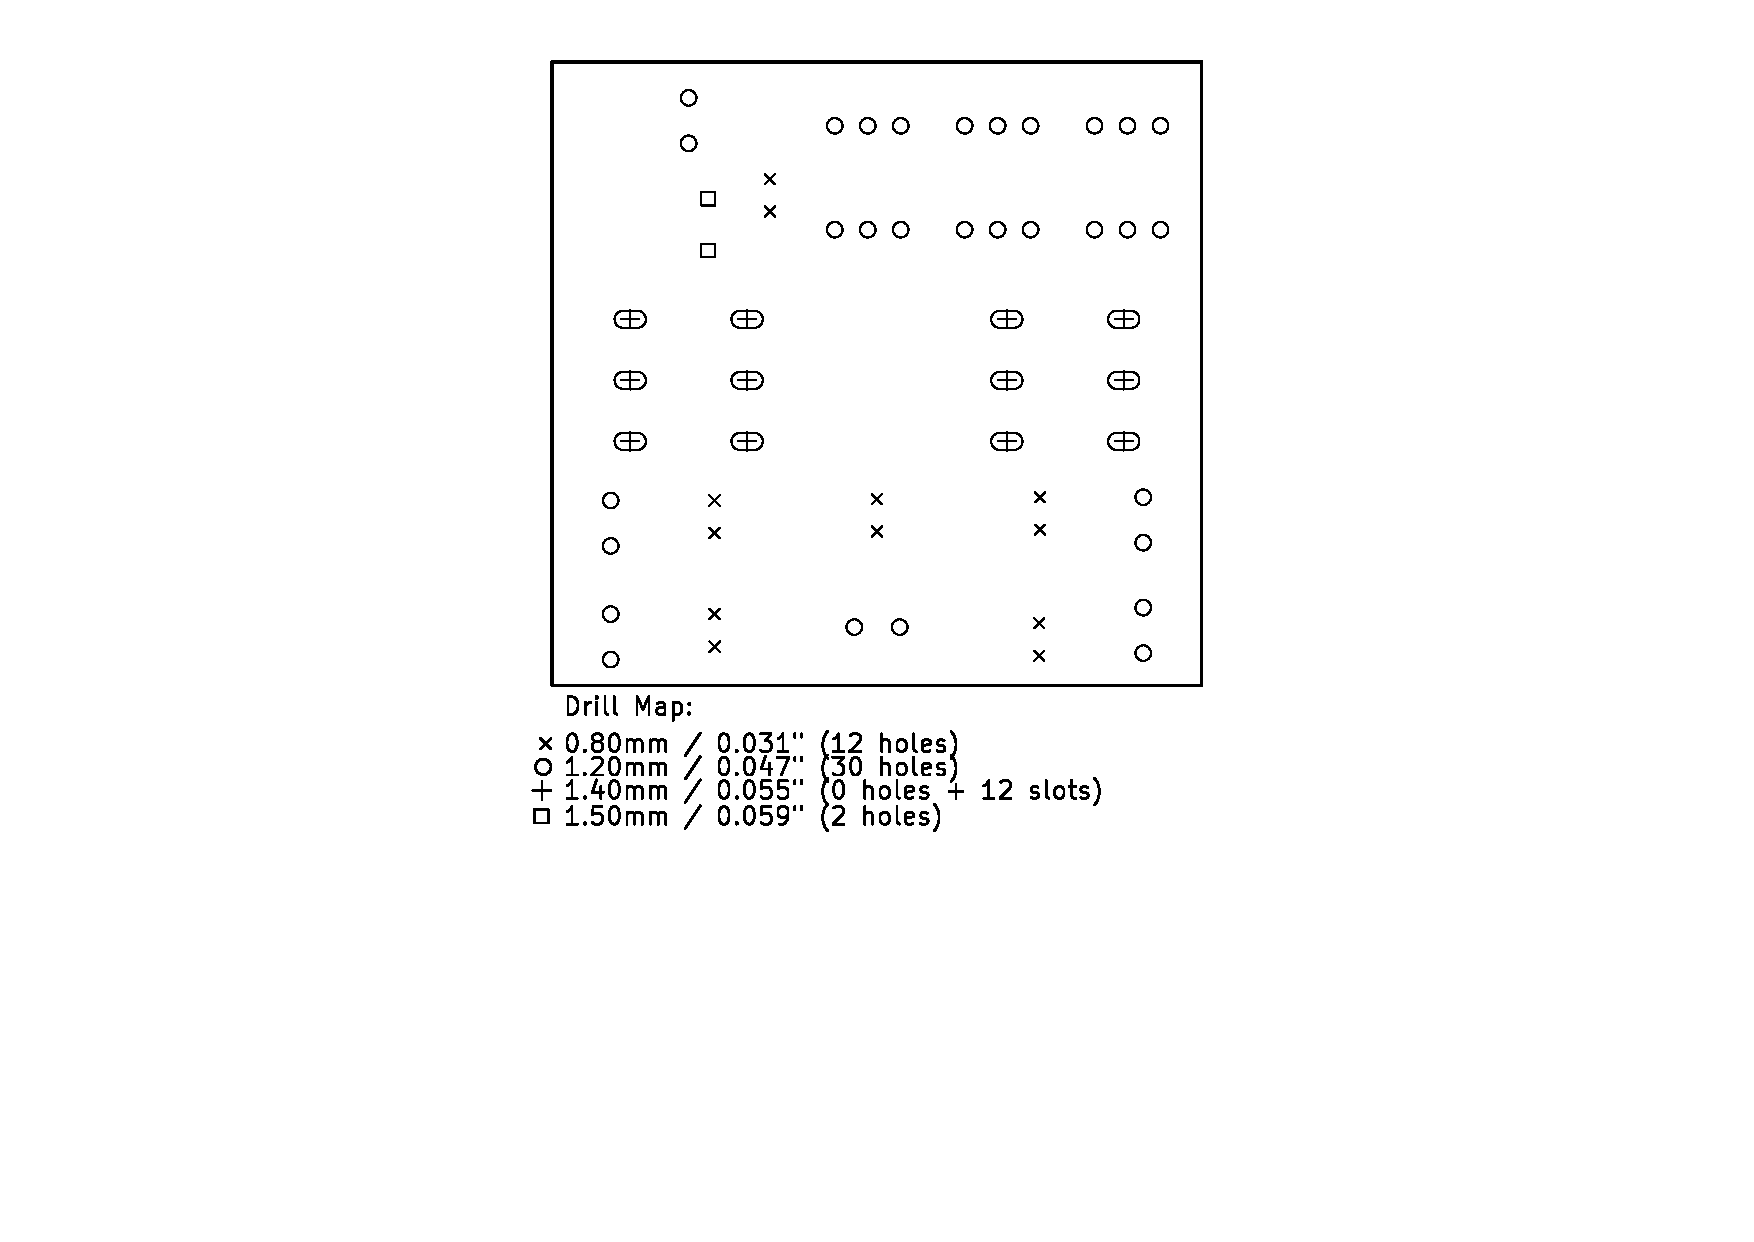
\includepdf[fitpaper]{inc/ccpdu_drill.pdf}
